\section{Conclusion}
\subsection{Future work}
\subsubsection{Path position leak}
In HOPR, payments are performed hop-by-hop along a packet’s route.
The incentives break the unlinkability guarantees inherited from the SPHINX packet format as they reveal the identity of the packet origin who transfers those incentives in the channel using their signature.
\\To solve this problem, HOPR forward incentives next to the packet.
\begin{figure}[H]
    \centering
    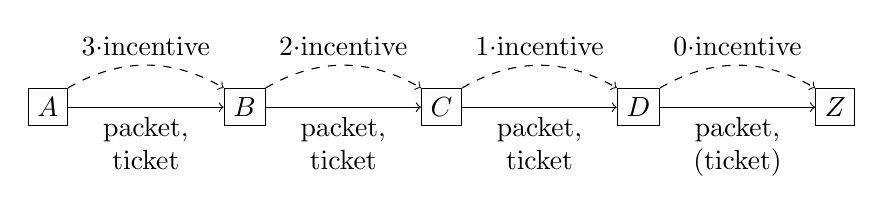
\begin{tikzpicture}[auto]
        \draw (0,0) node (a) [rectangle,draw] {$A$};
        \draw (2.5,0) node (b) [rectangle,draw] {$B$};
        \draw (5,0) node (c) [rectangle,draw] {$C$};
        \draw (7.5,0) node (d) [rectangle,draw] {$D$};
        \draw (10,0) node (z) [rectangle,draw] {$Z$};

        \draw [->,draw] (a.east) to node [align=center,below] {packet,\\ticket} (b.west);
        \draw [->,draw] (b.east) to node [align=center,below] {packet,\\ticket} (c.west);
        \draw [->,draw] (c.east) to node [align=center,below] {packet,\\ticket} (d.west);
        \draw [->,draw] (d.east) to node [align=center,below] {packet,\\(ticket)}  (z.west);

        \path [->,draw,bend left,dashed] (a.north east) to node [above] {3$\cdot$incentive} (b.north west);
        \path [->,draw,bend left,dashed] (b.north east) to node [above] {2$\cdot$incentive} (c.north west);
        \path [->,draw,bend left,dashed] (c.north east) to node [above] {1$\cdot$incentive} (d.north west);
        \path [->,draw,bend left,dashed] (d.north east) to node [above] {0$\cdot$incentive} (z.north west);

    \end{tikzpicture}    
    \caption{Incentive workflow}
    \label{fig:incentive worklow}
\end{figure}

\hspace{-5mm}This however leaks the relayer’s position within the selected path since the value of the ticket is set according to the current relay fee and the number of intermediate hops,
more precisely $$amount:=\frac{(hops -1)* relayFee}{winProb}$$
This leakage is considered to have a low severity but further research will be conducted on the subject.
\subsubsection{Reputation (aggregated trust matrix)}

In HOPR, we assume the majority of nodes are honest and act properly. Nevertheless, there might be nodes who actively try to attract the network by:
\begin{itemize}
    \item Dropping packets or acknowledgements
    \item Sending falsy packets, tickets or acknowledgements
\end{itemize}
Since nodes need to monitor the network to select paths, they need to filter nodes that behave inappropriately.
In order to do so, HOPR plans to implement a transitive reputation system which gives a score to each node that acts as a relayer.
\\The node’s reputation either increases or decreases its probability of being chosen depending on its behavior.

\subsubsection*{Transitive trust evaluation }
The reputation can be defined as: “a peer’s belief in another peer’s capabilities, honesty and reliability based on the other peers recommendations.”
Trust is represented by a triplet (trust, distrust, uncertainty) where:
\begin{itemize}
    \item Trust: $td^t(d,e,x,k)=\frac{n}{m}$ where $m$ is the number of all experiences and $n$ are the positive ones
    \item Distrust: $tdd^t(d,e,x,k)=\frac{l}{m}$ where $l$ stands for the number of the trustor’s negative experience.
    \item Uncertainty = 1 - trust - distrust.
\end{itemize}

